%%%%%%%%%%%%%%%%%%%%%%%%%%%%%%%%%%%%%%%%%%%%%%%%%%%%%%%%%%%%%%%%%%%%%
%% This is a (brief) model paper using the achemso class
%% The document class accepts keyval options, which should include
%% the target journal and optionally the manuscript type.
%%%%%%%%%%%%%%%%%%%%%%%%%%%%%%%%%%%%%%%%%%%%%%%%%%%%%%%%%%%%%%%%%%%%%
\documentclass[journal=jpcbfk,manuscript=article]{achemso}

%\documentclass[english,aps,preprint,pre,floatfix,nofootinbib,showpacs,showkeys]{revtex4-1}
%%%%%%%%%%%%%%%%%%%%%%%%%%%%%%%%%%%%%%%%%%%%%%%%%%%%%%%%%%%%%%%%%%%%%
%% Place any additional packages needed here.  Only include packages
%% which are essential, to avoid problems later. Do NOT use any
%% packages which require e-TeX (for example etoolbox): the e-TeX
%% extensions are not currently available on the ACS conversion
%% servers.
%%%%%%%%%%%%%%%%%%%%%%%%%%%%%%%%%%%%%%%%%%%%%%%%%%%%%%%%%%%%%%%%%%%%%
\usepackage[version=3]{mhchem} % Formula subscripts using \ce{}

\SectionNumbersOn

\usepackage{amsmath}
\usepackage{amssymb}
\usepackage{color}
\usepackage{CJK}https://www.overleaf.com/project/5e820b28d741e00001b1ccac
\usepackage{framed}
\usepackage[hidelinks]{hyperref}
\usepackage{algorithm}
\usepackage{algpseudocode}
\algdef{SE}[DOWHILE]{Do}{doWhile}{\algorithmicdo}[1]{\algorithmicwhile\ #1}

\usepackage[scaled=0.85]{beramono}
\usepackage[T1]{fontenc}
\usepackage{changepage}

%%%%%%%%%%%%%%%%%%%%%%%%%%%%%%%%%%%%%%%%%%%%%%%%%%%%%%%%%%%%%%%%%%%%%
%% If issues arise when submitting your manuscript, you may want to
%% un-comment the next line.  This provides information on the
%% version of every file you have used.
%%%%%%%%%%%%%%%%%%%%%%%%%%%%%%%%%%%%%%%%%%%%%%%%%%%%%%%%%%%%%%%%%%%%%
%%\listfiles

%%%%%%%%%%%%%%%%%%%%%%%%%%%%%%%%%%%%%%%%%%%%%%%%%%%%%%%%%%%%%%%%%%%%%
%% Place any additional macros here.  Please use \newcommand* where
%% possible, and avoid layout-changing macros (which are not used
%% when typesetting).
%%%%%%%%%%%%%%%%%%%%%%%%%%%%%%%%%%%%%%%%%%%%%%%%%%%%%%%%%%%%%%%%%%%%%

\makeatletter
    \setlength\@fptop{0\p@}
\makeatother

\newcommand*\mycommand[1]{\texttt{\emph{#1}}}

\newcommand{\state}[1]{$\mathcal{S}_{#1}$}

%\newcommand*{\rood}[1]{\textcolor{red}{#1}}
\newcommand*{\rood}[1]{#1}
%\newcommand*{\blauw}[1]{\textcolor{blue}{#1}}
\newcommand*{\blauw}[1]{#1}
%\newcommand*{\groen}[1]{\textcolor{green}{#1}}
\newcommand*{\groen}[1]{#1}
%\newcommand*{\blauwr}[1]{\textcolor{blue}{#1}}
\newcommand*{\blauwr}[1]{#1}

%\newcommand*{\addref}[1]{\textcolor{red}{\{ADD REF: #1\}}}

%\newcommand*{\noter}[1]{\textcolor{red}{[[#1]]}}		% notes on
\newcommand*{\noter}[1]{}					% notes off

%\usepackage[draft]{todonotes}   % notes shown
\usepackage[disable]{todonotes} % notes hidden

%%%%%%%%%%%%%%%%%%%%%%%%%%%%%%%%%%%%%%%%%%%%%%%%%%%%%%%%%%%%%%%%%%%%%
%% Meta-data block
%% ---------------
%% Each author should be given as a separate \author command.
%%
%% Corresponding authors should have an e-mail given after the author
%% name as an \email command. Phone and fax numbers can be given
%% using \phone and \fax, respectively; this information is optional.
%%
%% The affiliation of authors is given after the authors; each
%% \affiliation command applies to all preceding authors not already
%% assigned an affiliation.
%%
%% The affiliation takes an option argument for the short name.  This
%% will typically be something like "University of Somewhere".
%%
%% The \altaffiliation macro should be used for new address, etc.
%% On the other hand, \alsoaffiliation is used on a per author basis
%% when authors are associated with multiple institutions.
%%%%%%%%%%%%%%%%%%%%%%%%%%%%%%%%%%%%%%%%%%%%%%%%%%%%%%%%%%%%%%%%%%%%%
\author{Mike Jones}
\affiliation{%
  Pritzker School of Molecular Engineering, %
  University of Chicago, %
  Chicago, Illinois 60637%
}

\author{Andrew L. Ferguson}
\email{andrewferguson@uchicago.edu}
\affiliation{%
  Pritzker School of Molecular Engineering, %
  University of Chicago, %
  Chicago, Illinois 60637%
}
%\author{I. Ken Groupleader}
%\altaffiliation{A shared footnote}
%\email{i.k.groupleader@unknown.uu}
%\phone{+123 (0)123 4445556}
%\fax{+123 (0)123 4445557}
%\affiliation[Unknown University]
%{Department of Chemistry, Unknown University, Unknown Town}
%\alsoaffiliation[Second University]
%{Department of Chemistry, Second University, Nearby Town}

%\author{Susanne K. Laborator}
%\email{s.k.laborator@bigpharma.co}
%\affiliation[BigPharma]
%{Lead Discovery, BigPharma, Big Town, USA}

%\author{Kay T. Finally}
%\affiliation[Unknown University]
%{Department of Chemistry, Unknown University, Unknown Town}
%\alsoaffiliation[Second University]
%{Department of Chemistry, Second University, Nearby Town}

%%%%%%%%%%%%%%%%%%%%%%%%%%%%%%%%%%%%%%%%%%%%%%%%%%%%%%%%%%%%%%%%%%%%%
%% The document title should be given as usual. Some journals require
%% a running title from the author: this should be supplied as an
%% optional argument to \title.
%%%%%%%%%%%%%%%%%%%%%%%%%%%%%%%%%%%%%%%%%%%%%%%%%%%%%%%%%%%%%%%%%%%%%
\title[]{TBA}


%%%%%%%%%%%%%%%%%%%%%%%%%%%%%%%%%%%%%%%%%%%%%%%%%%%%%%%%%%%%%%%%%%%%%
%% Some journals require a list of abbreviations or keywords to be
%% supplied. These should be set up here, and will be printed after
%% the title and author information, if needed.
%%%%%%%%%%%%%%%%%%%%%%%%%%%%%%%%%%%%%%%%%%%%%%%%%%%%%%%%%%%%%%%%%%%%%
%\abbreviations{IR -- infrared, NMR -- nuclear magnetic resonance, UV -- ultraviolet}
%\keywords{Takens}

\begin{document}
%%%%%%%%%%%%%%%%%%%%%%%%%%%%%%%%%%%%%%%%%%%%%%%%%%%%%%%%%%%%%%%%%%%%%
%% The manuscript does not need to include \maketitle, which is
%% executed automatically.  The document should begin with an
%% abstract, if appropriate.  If one is given and should not be, the
%% contents will be gobbled.
%%%%%%%%%%%%%%%%%%%%%%%%%%%%%%%%%%%%%%%%%%%%%%%%%%%%%%%%%%%%%%%%%%%%%

\newpage

\begin{abstract}

\noindent 

\end{abstract}
https://www.overleaf.com/project/5e9e5110c524b8000192c548
%%%%%%%%%%%%%%%%%%%%%%%%%%%%%%%%%%%%%%%%%%%%%%%%%%%%%%%%%%%%%%%%%%%%%
%% Start the main part of the manuscript here.
%%%%%%%%%%%%%%%%%%%%%%%%%%%%%%%%%%%%%%%%%%%%%%%%%%%%%%%%%%%%%%%%%%%%%

\newpage

\section{\label{sec:intro}Introduction}
Should be 4-5 paragraphs with similar structure to other papers in the field.
-Funnel shaped to highlight general DNA technologies (oligomers and 

\subsection{\label{sec:intro}DNA motivation}
\subsubsection{\label{sec:intro}Main Question: how does sequence determine the kinetics of DNA oligonucleotides}

\subsubsection{\label{sec:intro}What is known about the system and what remains an open question -- reference Tokmakoff frayed states here}

\subsubsection{\label{sec:intro}Thermodynamics are well established and some MSM based (high resolution kinetic) models have been employed to study kinetics}

\subsubsection{\label{sec:intro}Circle back to applications after discussing the open question that we are seeking to solve -- how does this expand on existing technolgies}

\subsection{\label{sec:intro}SRV motivation}
\subsubsection{\label{sec:intro}First time studying a two body problem}
\subsubsection{\label{sec:intro}Compare with other TICA-MSM approaches to DNA}

Over the last couple decades, DNA has proved to be much more than a vessel for genetic information. From sensing, to computing, to directed self-assembly, the programmable and predictable nature of DNA has unlocked numerous unforeseen applications \citep{Seeman2017DNANanotechnology} (cite more). Recently, structural DNA nanotechnology has enabled self-assembly on micro to milli scales \citep{MhatreV.HoJi-AnnLee2012NIHAccess}, and dynamic DNA nanotechnology has been used to perform basic calculation \citep{Bui2018} and to probe single molecules via temporal DNA signatures \citep{Shah2019}. Both technologies rely on the hybridization reaction between complementary (or similar) DNA strands and leverage the flexibility of shorter DNA oligomers to participate in these reactions. Although many experimental and computational studies have been performed to investigate hybridization and dissociation, the sequence-dependent mechanisms of hybridization dynamics are not fully understood (cite). Moreover, it is unclear whether these processes occur in an "all-or-nothing" fashion or if some metastable states can facilitate the process. The stability of out of register or "slipped" base pairing in repetitive sequences has been well documented in previous computational studies \citep{Phys2014}, \citep{Xiao2019}) and are referred to as slip-strand DNA for longer seqeunces in vivo (cite, maybe too unrelated). Sandstead et al suggested the existence of frayed metastable states during duplex dissociation, where the stability of these states was dictated by oligonucleotide sequence \citep{Sanstead2016}. In this work, we study the same four sequences explored by Sandstead et al in an effort to uncover the sequence-dependent dynamics and their relation to  metastable structures mentioned above.

Given the long timescales on which DNA hybridization and dissociation events occur, the study of these processes are generally not amenable to direct simulation techniques \citep{Phys2014}. Instead, many previous studies of DNA hybridization have employed accelerated sampling methods such as umbrella sampling \citep{Schmitt2013ExploringSurface} transition path sampling \citep{Sambriski2009}, \citep{Hoefert2011MolecularOligonucleotides}  and forward flux sampling  \citep{Phys2014} (cite more). In this work, we leverage the properties of Markov State Models (MSMs) -- namely that conditional probability depends only on the current state of the system \citep{Pande2010EverythingAsk}--  to run many unbiased coarse-grained simulations and combine these independent simulations to form an understanding of the kinetics and thermodynamics. MSMs have been used recently to study mechanisms of DNA hybridization  \citep{Jin2019} \citep{Xiao2019}, but the slowest sequence-dependent kinetics were not the focus of these studies. Pinamonti et al. used MSMs to compare the slowest dynamics of short RNA nucleotides and found that stacking timescales are highly sequence dependent \citep{Pinamonti2017}. We take a similar approach to study 10-mer DNA oligonucleotides and introduce State Reversible Vampnets (SRVs) to directly learn the slowest sequence-dependent dynamical modes \citep{Chen}. Furthermore, we integrate SRVs into the MSM pipeline by generating an optimized low dimensional basis in which microstates clustering can be performed. We show that SRV coordinates can be useful for both directly interpreting dynamical trends and for improving overall MSM quality when compared to more conventional methods such as Time-structure independent components analysis (tICA).

Our analysis reflects similar results to previous computational and experimental DNA work, while elucidating some new insights into sequences dependent dynamics and relative timescales. (something here about how this could motivate future experimental work or applications?) By employing SRVs to generate an optimized low dimensional basis, we can access higher resolution MSMs (shorter lag time) and generate a more detailed model. The slow dynamical modes learned by SRVs can be directly compared between sequences to determine otherwise subtle trends. Furthermore, this work represents the first application of SRVs to a two-body system -- in particular a system that includes permutable distances. Our results suggest that this will be a promising tool to study future two-body or many-body molecular dynamics systems.

\section{\label{sec:methods}Methods}

\subsection{\label{sec:methods}Previous feedback and advice} 

-don't confuse methods plots with results
-not necessary to plot vamp-2 scores (or can include comaprisons in the SI)
-follow basic outline of Trp-Cage methods in the order sim, srv, msm (a lot of the msm will be in results, but can go through basic assumptions and pytemma pipeline)
-less of a narrative and more of an assertive manner

\subsection{\label{sec:methods}Notes and questions} 
Trp-Cage paper did not really have a dedicated methods section, so basing this more on other papers.

\subsection{\label{sec:methods}Simulation set up}
\subsubsection{\label{sec:methods}Tmelt selection etc}

We initialized four sequences previously investigated by Sandstead et al \citep{Sanstead2016} -- AT-all, GC-core, GC-end, and GC-mid -- (small figure here) along with their complementary strands according to 3SPN.2 documentation \citep{Phys2014}. We initialized explicit ions such that 240 mM NaCl and 18 mM MgCl2 were added to the box in addition to 18 Na counter ions to balance the charge from the 9 phosphate groups in each oligonucleotide backbone \citep{Hinckley2015}. In order to maximize concentration without allowing strands to see each other through periodic boundaries, we set the box size just larger than the sum of the maximum end to end extension length of a single strand and the force cutoff (using Ewald summation method is set at 20 A). This translated to a box size of 77.74 A and an effective oligo concentration of 7 mM. We used an Ewald potential to calculate long range 
Coulombic interaction between DNA and ions. We maintained a Debye-Huckel screening potential with an ionic strength of 240 mM -- corresponding to NaCl concentration -- to account for phosphate backbone interactions. These electrostatics preserve the persistence length and intrinsic curvature of DNA while taking the effects of ion-DNA interactions\citep{Hinckley2015}. A 15 fs timestep was used for all simulations runs.

Simulation temperature was determined by sequence specific melting temperature (Tmelt selection). Tmelt simulations were run for $3*10^{8}$ time steps, equating to 4.5$\mu$s simulation time, and frames were saved every 30 ps. For each sequences, 100 simulations were performed in parallel, consuming about 32 serial cpu-hours of computation time for each independent simulation. An approximate Tmelt Boltzman distribution was replicated by initializing half of runs from the hybridized state and half from a random dissociated state. In order to allow for further equilibration, the first third (1.5 $\mu$s) of each simulation was removed, resulting in 100 x 100000 frames and a total of 300$\mu$s simulation time per sequence.

\begin{figure}[ht!]
	\begin{center}
        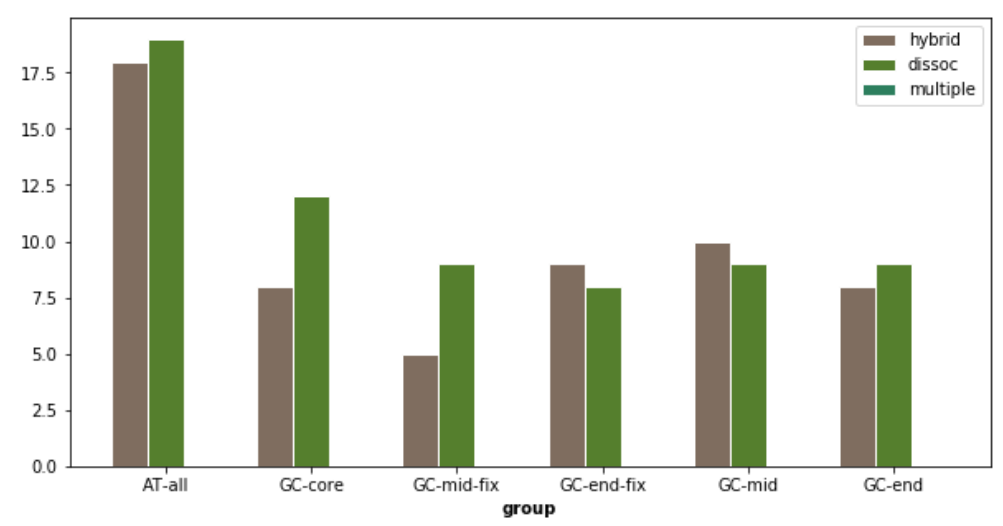
\includegraphics[width=\textwidth]{Figs/skeleton/n_events.PNG}
        \caption{Number of events per sequence. I would only included the four sequences in the actual pub. (this could be supplemental}
        \label{fig:n_events}
	\end{center}
\end{figure}   

\subsection{\label{sec:methods}SRV}
\subsubsection{\label{sec:methods}Featurization}

\begin{enumerate}
	\item Vamp-2 score for permutable distances is slightly lower but should not contain degenerate information (SI data)
	\item Inverse distances have higher vamp-2 score than regular distances (SI data)
\end{enumerate}

All intermolecular pairwise distances for both oligonucleotides were calculated at each frame. Based on the self-complementary nature of each sequence, we averaged permutable distances (45 pairs in total) together. This permutation reduction follows a similar procedure used in TICAgg coordinates construction \citep{Sengupta2019AutomatedSelf-assembly}. The VAMP-2 scoring method, which represents the sum of squared estimates for the transfer operator, was employed to evaluate the quality of this feature set \citep{Mardt2018VAMPnetsKinetics}. We compared the VAMP-2 score (SI ?) for the permutation-free distances to the complete set of intermolecular distances and found only a small loss in kinetic variance when using the reduced data set. Furthermore, we found an increase in VAMP-2 score when using reciprocal pairwise distances and chose these reciprocal permutation-free coordinates as a consistent feature set. These features were normalized and passed into sequence-specific SRVs. 

\subsubsection{\label{sec:methods}Select number of slow modes (different for each) and lag (same for each) based on this analysis}

Using optimized hyperparameters and featurized trajectory data, we generated a hierarchical dynamic encoder (HDE) to transform 55 reciprocal pairwise distances into a low dimensional SRV feature set. In order to maintain consistency between sequences, we kept all training hyperparameters the same between SRVs with the exception of the number of outputed slow modes. An 80/20 validation split was used during training, and early stopping was implemented in Keras in order to halt training when validation loss was be minimized. SRV training required about 22 GPU-minutes across 1 GPU and 10 CPUs. (Should use cross-validation to prove with results were significant here).

**Describe selection of slow modes for each sequence first, then can talk about how we ensure an appropriate lag time is selected. Lag time was determine by looking for the shortest time at which all relevant slow modes had converged. We found that the leading slow mode took substantially longer to converge than higher order modes and did not include this mode in our metric for convergence.

\subsection{\label{methods}MSM construction}
\begin{enumerate}
	\item hyperparameters include: number of microstates, lag (use same as SRV), number of macrostates (usually n+1) but we use n states for GC-core and GC-mid. I have not done a full optimization sweep over these parameters, but can explain the motivation for choosing these.
    \item Can show comparison data with TICA -- timescales converge faster and state assignments tend to be more concrete (although this has varied) 
    \item As we discussed, I think a lot of this could got into the results, so I'm not exactly sure what to include in the methods
\end{enumerate} 

We employed the Pyemma Markov State Model (MSM) pipeline to analyze sequence-specific SRV coordinates. Again, we maintained as many hyperparameters consistent as possible between sequences in order to facilitate comparability. Using the SRV coordinates as a basis, kmeans clustering was used to group data into microstates where the number of microstates was optimized via VAMP-2 score. The score for each sequence leveled off around 200 microstates, and clustering in SRV space consistently yielded a high VAMP-2 score than clustering in TICA space (SI fig). Next, implied timescales were estimated over a range of lag times based on these discretized states. We then looked for an MSM lag time that was both Markovian and capable of resolving as much detail as possible. We found that SRV timescales converged consistently faster and to higher values than TICA. Because these timescales are underestimates for the true timescales of the system, we can assume that SRV coordinates are better at both capturing dynamics and enabling better resolution for MSM construction. Bayesian Markov Models were constructed from both SRV and TICA clusters, and PCCA+ clustering was performed for macrostates assignment. The procedure for determining the number of PCCA cluster centers was performed on a sequence specific basis and will be discussed in the results section.

** The above paragraph is definitely blending into results, not sure how much exactly to include. It might be easier to to use AT-all as a case study for explaining the overall process, but the those results are pretty distinct from other sequences so I don't want it to be misleading.

\begin{figure}[ht!]
	\begin{center}
        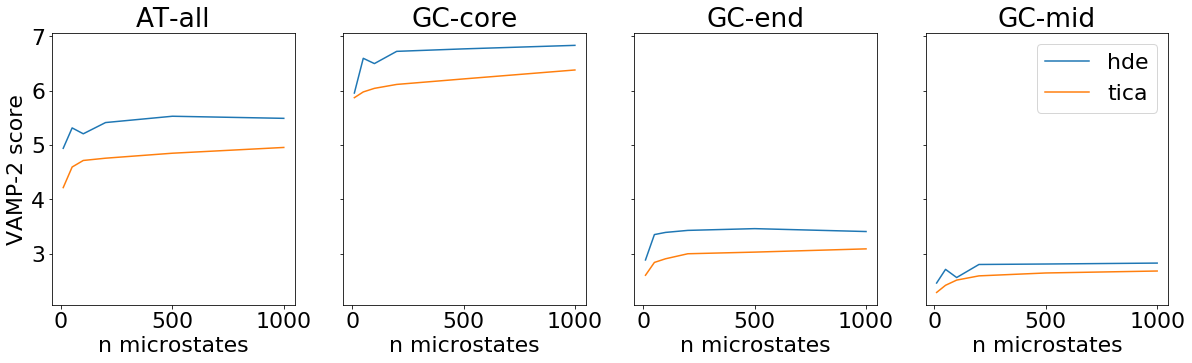
\includegraphics[width=\textwidth]{Figs/skeleton/microstate_optimization.png}
        \caption{Finding optimal amount of microstates for SRV and TICA clustering. VAMP-2 scores are consistently higher when clustering in SRV space}
        \label{fig:sample_fray}
	\end{center}
\end{figure}


\section{\label{sec:Results}Results}
- lead with same kind of diagram for each sequence, add additional figures when necessary for a given sequence

\subsection{\label{sec:Results}AT-all}
\subsubsection{\label{sec:Results}Explanation of state selection and slow modes}
\subsubsection{\label{sec:Results}Brief description and diagrams for collective variables}
\begin{enumerate}
	\item Inverse average shifting distance
	\item Fourth basepair distances
\end{enumerate} 

\begin{figure}[ht!]
	\begin{center}
        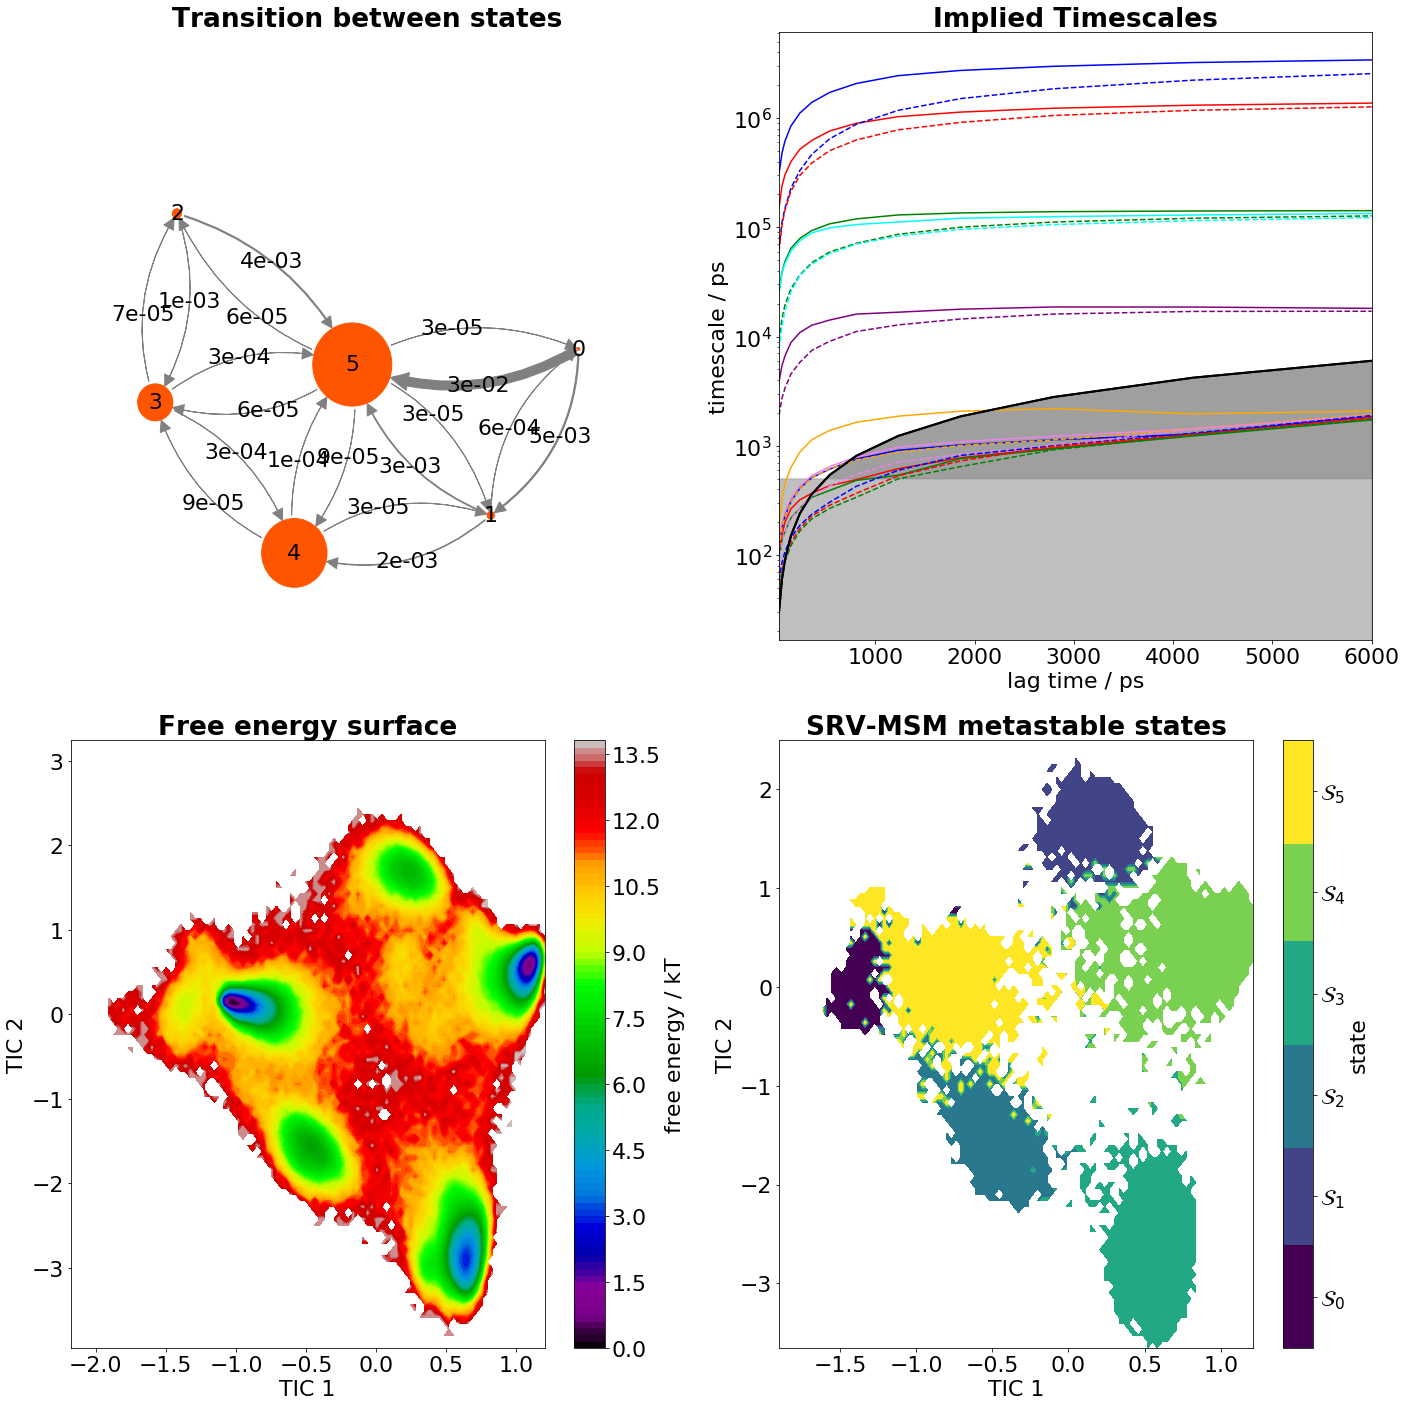
\includegraphics[width=\textwidth]{Figs/skeleton/AT-all_vis.png}
        \caption{AT-all transition diagram, implied timescales between SRV-MSM and TICA-MSM, free energy surface and metastable state assignment.}
        \label{fig:sample_fray}
	\end{center}
\end{figure}

\subsubsection{\label{sec:Results}Observations and key takeaways}
\begin{enumerate}
	\item Dynamics dominated by slow shifting modes
	\item sources to verify this would be the case
	\item Minimal data from Tokmakoff on this, but can look at relative hybridization rates
	\item SI Calculations to prove preferred thermo stability of 5’ shifted state
\end{enumerate}  

\subsection{\label{sec:Results}GC-end}
\begin{enumerate}
	\item Similar dynamics to AT-all, but with overall lower stability and timescales
	\item Difficult to make any claims because the thermodynamics of external mismatches with dangling ends have not been measured experimentally, and 3spn2 does not paramertize these mismatches explicitly
	\item According to SantaLucia external mismatches and dangling ends tend to have weakly stabilizing effect, and there are 4-6 intact basepairs for these conformations
	\item Might account for unknown signal in 2018 Tokmakoff paper with timescale between the fraying and dehybrization signal, but not sure... 
\end{enumerate}  

\begin{figure}[ht!]
	\begin{center}
        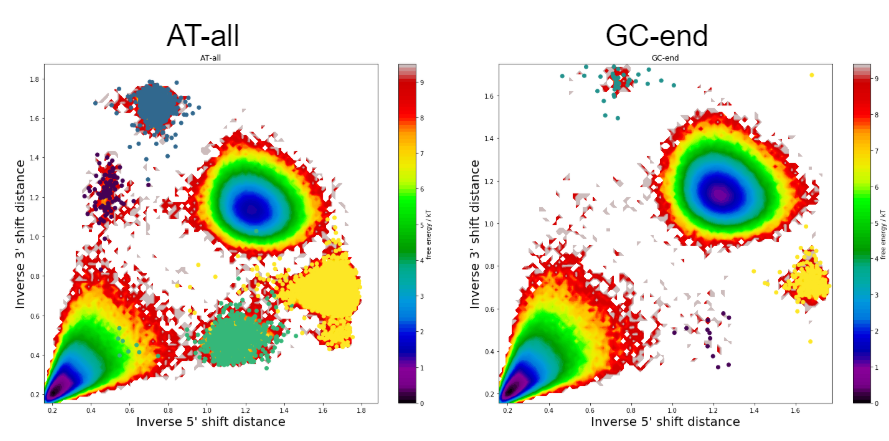
\includegraphics[width=\textwidth]{Figs/skeleton/shifting_distribution.PNG}
        \caption{Shows similarities between shifting modes and state memberships for AT-all and GC-ends}
        \label{fig:shifting_distributions}
	\end{center}
\end{figure}

\subsection{\label{sec:Results}GC-core}
\begin{enumerate}
	\item Frayed states requires the fourth base pair to be broken, most partially frayed states are not included in metastable clustering
	\item 2nd slow mode correlates well with expected fraying behavior, can sample along this mode and generally find increasing frayed states (although the SRV coords are spiky)
	\item 3rd mode is reflective of changes in orientation in dissociated behavior. This could be interesting for the SI, but this state does not inform the macrostate clustering
\end{enumerate}

\begin{figure}[ht!]
	\begin{center}
        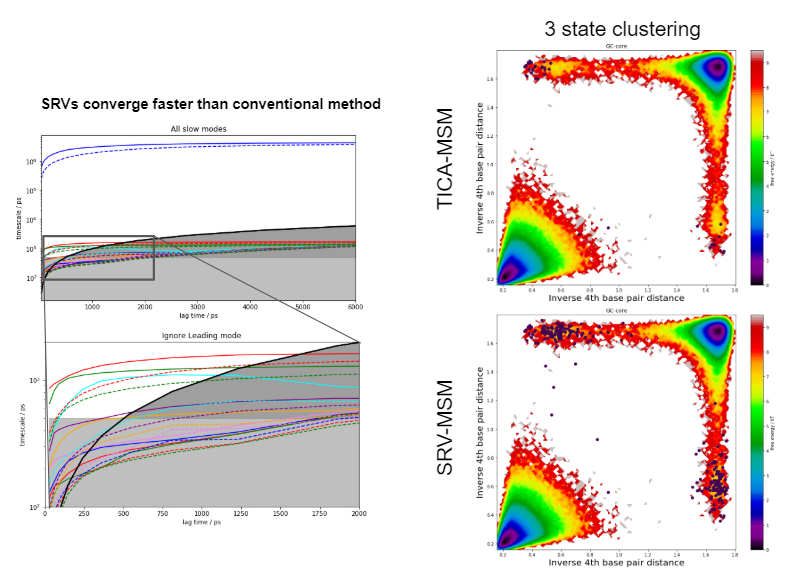
\includegraphics[width=\textwidth]{Figs/skeleton/tica_comparison_GC-core.PNG}
        \caption{SRV vs. TICA MSMs and resulting clsuter memberships}
        \label{fig:tica_comparison}
	\end{center}
\end{figure}

\begin{figure}[ht!]
	\begin{center}
        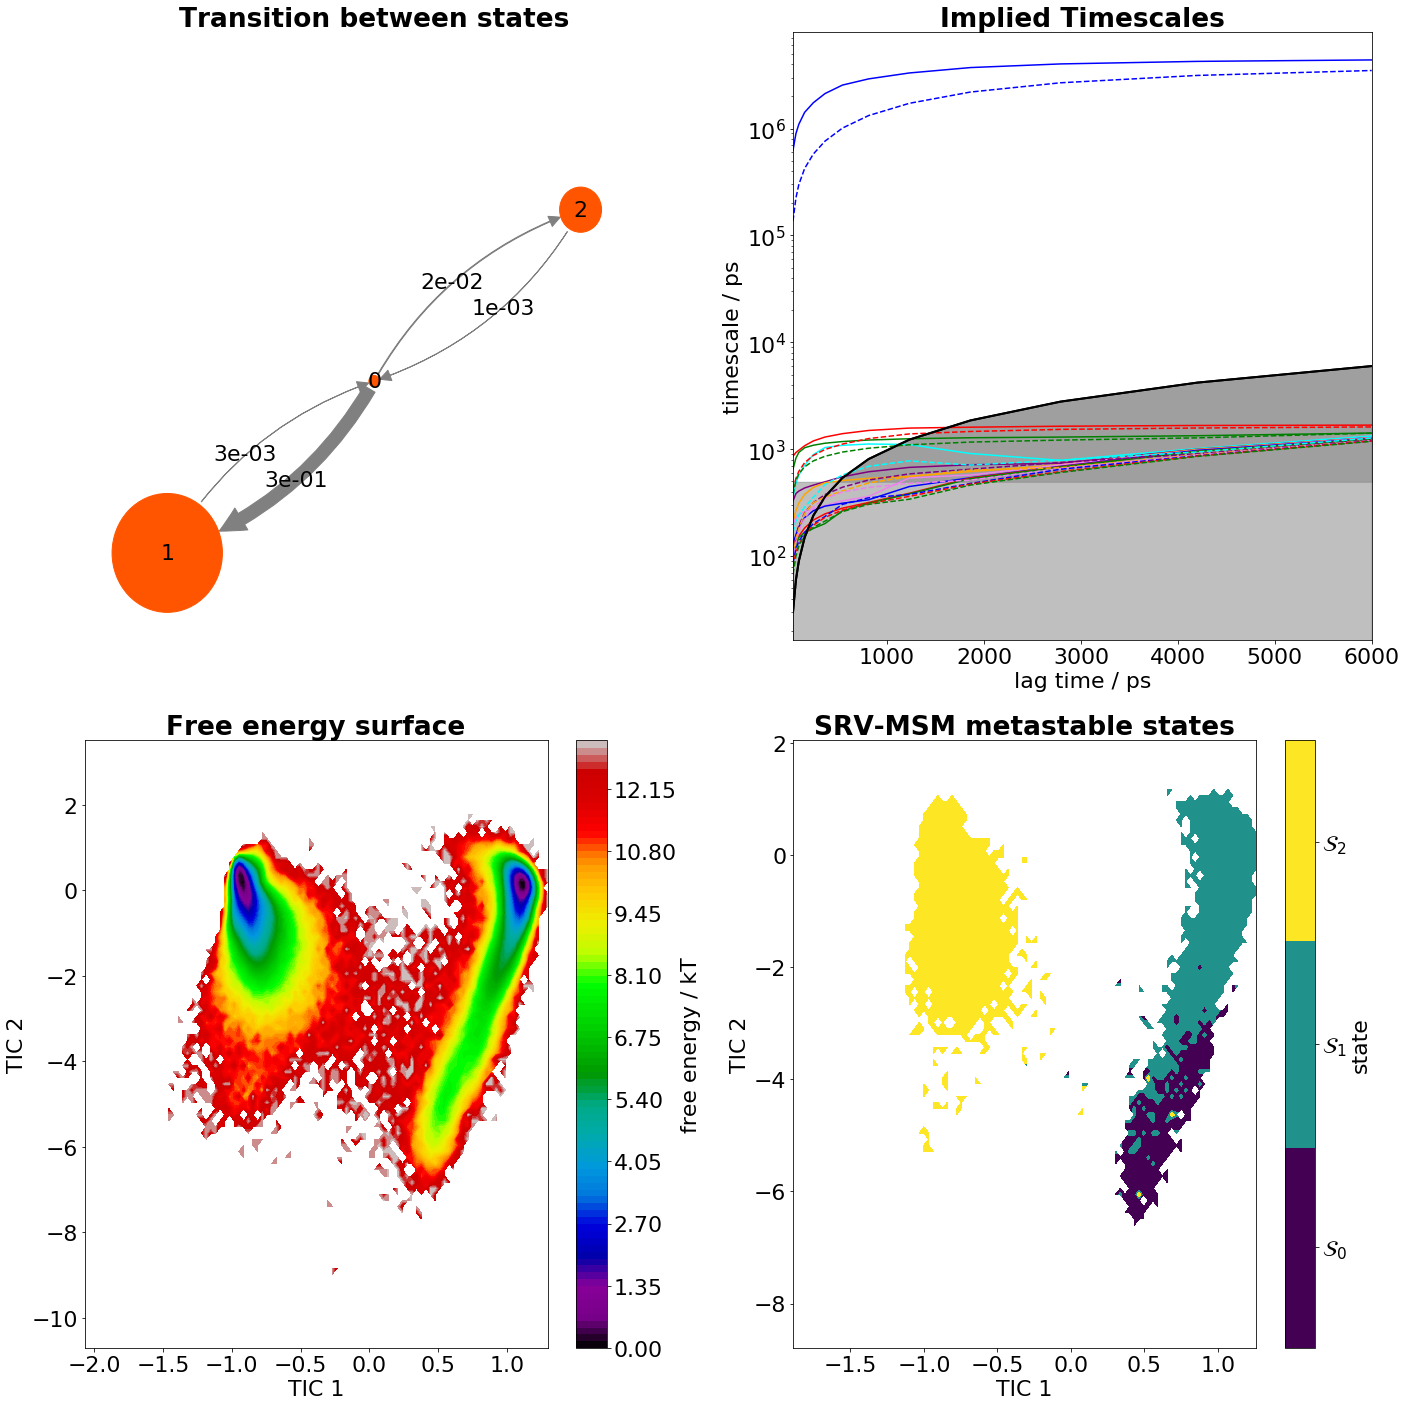
\includegraphics[width=\textwidth]{Figs/skeleton/GC-core_vis.png}
        \caption{GC-core transition diagram, implied timescales between SRV-MSM and TICA-MSM, free energy surface and metastable state assignment.}
        \label{fig:sample_fray}
	\end{center}
\end{figure}

\begin{figure}[ht!]
	\begin{center}
        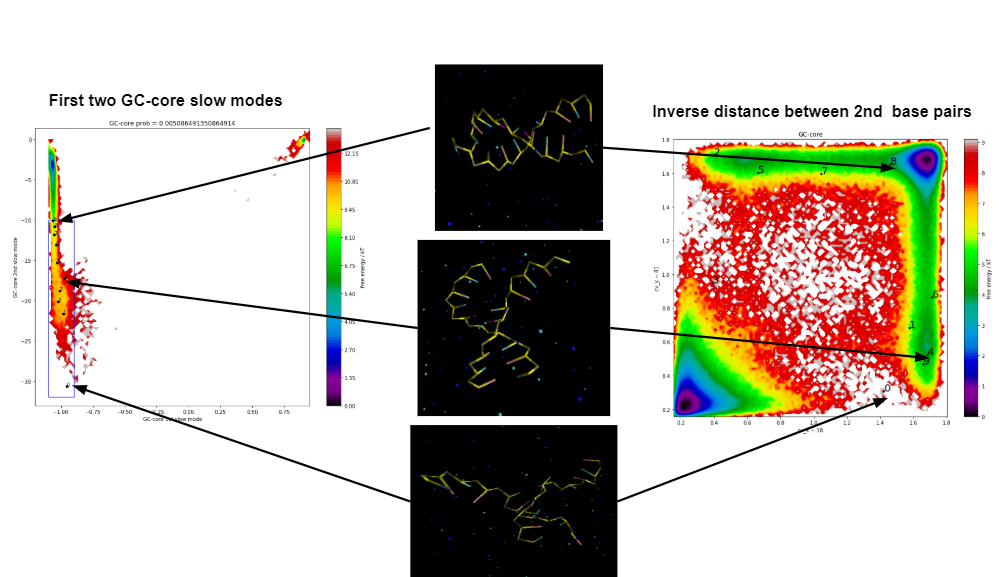
\includegraphics[width=\textwidth]{Figs/skeleton/sample_fray.PNG}
        \caption{Sample along 2nd GC-core SRV mode and show that these have increasing amounts of fraying}
        \label{fig:sample_fray}
	\end{center}
\end{figure}

\subsection{\label{sec:Results}GC-mid}
\begin{enumerate}
	\item Evidence of fraying correlations in higher order modes, but these are not consistent and their inclusion does not generate a metastable third mode
	\item Treat this as a two-states model, where fraying is an expected feature of the hybridized state but not does not characterize a metastable state
\end{enumerate}  

\subsection{\label{sec:Results}Compare all results together}
\subsubsection{\label{sec:Results}Figure showing Pearson correlations between leading modes on common basis}

\begin{figure}[ht!]
	\begin{center}
        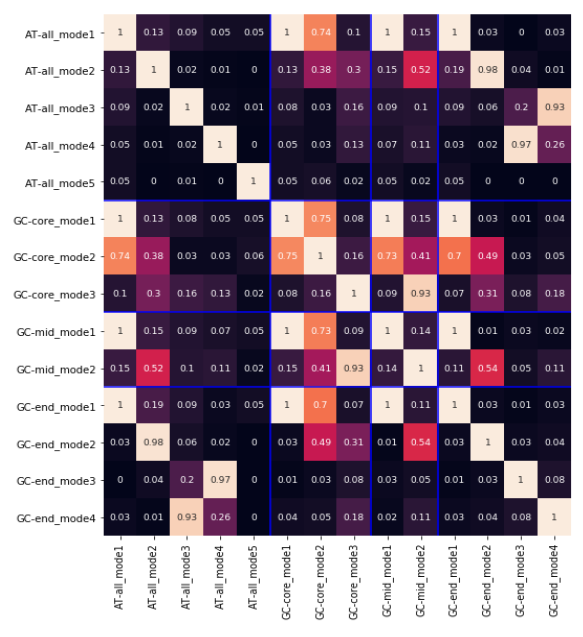
\includegraphics[width=\textwidth]{Figs/skeleton/all_modes_correlations.PNG}
        \caption{For Supplemental info: Correlations between all leading modes}
        \label{fig:all_modes}
	\end{center}
\end{figure}

\subsubsection{\label{sec:Results}Figure showing all sequences plotted on a common low dimensional space (probably the 2nd TICA mode and the 2nd GC-core mode)}

\begin{enumerate}
	\item Evidence of fraying correlations in higher order modes, but these are not consistent and their inclusion does not generate a metastable third mode
	\item Treat this as a two-states model, where fraying is an expected feature of the hybridized state but not does not characterize a metastable state
\end{enumerate}
    
\section{\label{sec:conc}Conclusion}
\subsection{\label{sec:Results}Looks a lot like the abstract}
    
    
\section{\label{sec:SI}Potential SI figures}
\begin{figure}[ht!]
	\begin{center}
        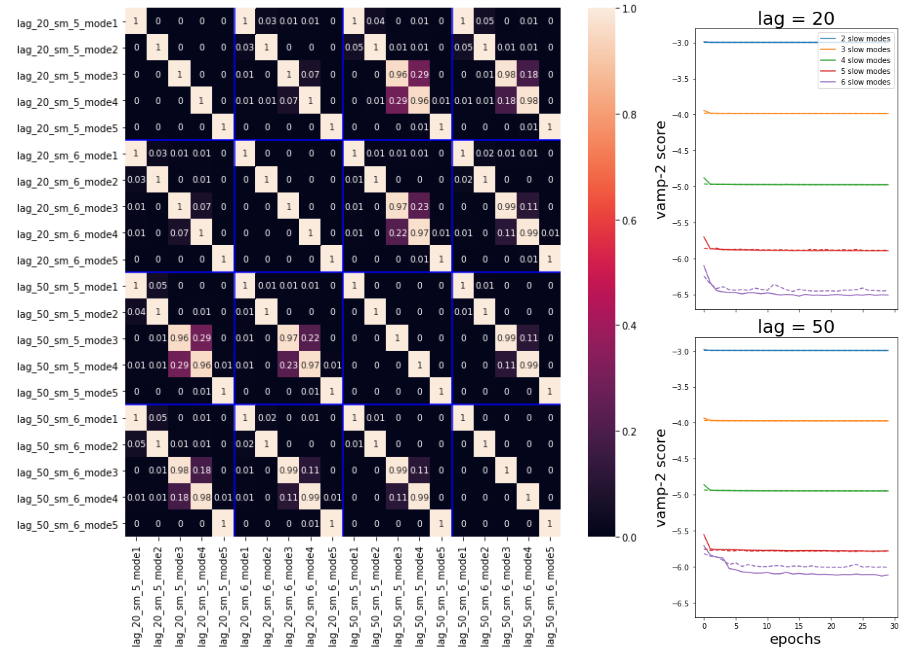
\includegraphics[width=\textwidth]{Figs/skeleton/AT-all_validation.PNG}
        \caption{For Supplemental info: Selection process for AT-all slow modes}
        \label{fig:AT-all_val}
	\end{center}
\end{figure}

\begin{figure}[ht!]
	\begin{center}
        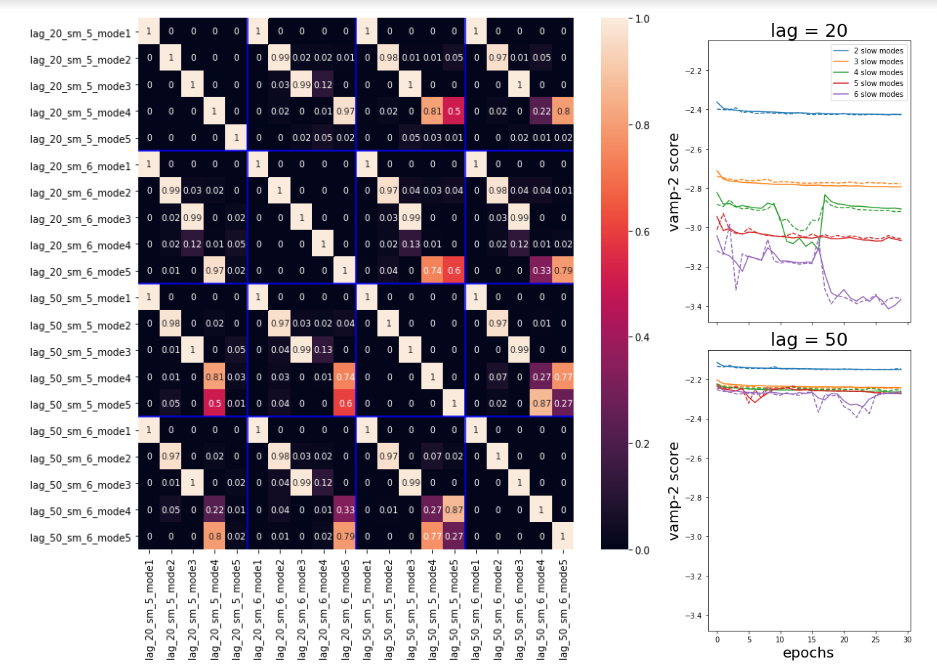
\includegraphics[width=\textwidth]{Figs/skeleton/GC-core_validation.PNG}
        \caption{For Supplemental info: Selection process for GC-core slow modes}
        \label{fig:GC-core_val}
	\end{center}
\end{figure}


\clearpage
\newpage

%\bibliography{references}
Test cite: \citep{Zhang2018DeepMechanics}
\bibliography{refs_mendeley}

%%%%%%%%%%%%%%%%%%%%%%%%%%%%%%%%%%%%%%%%%%%%%%%%%%%%%%%%%%%%%%%%%%%%%
%% The "tocentry" environment can be used to create an entry for the
%% graphical table of contents.
%%%%%%%%%%%%%%%%%%%%%%%%%%%%%%%%%%%%%%%%%%%%%%%%%%%%%%%%%%%%%%%%%%%%%

\clearpage


\end{document}
